\chapter{Frontend}

%login
\section{Login}
\begin{figure}[h]
    \centering
    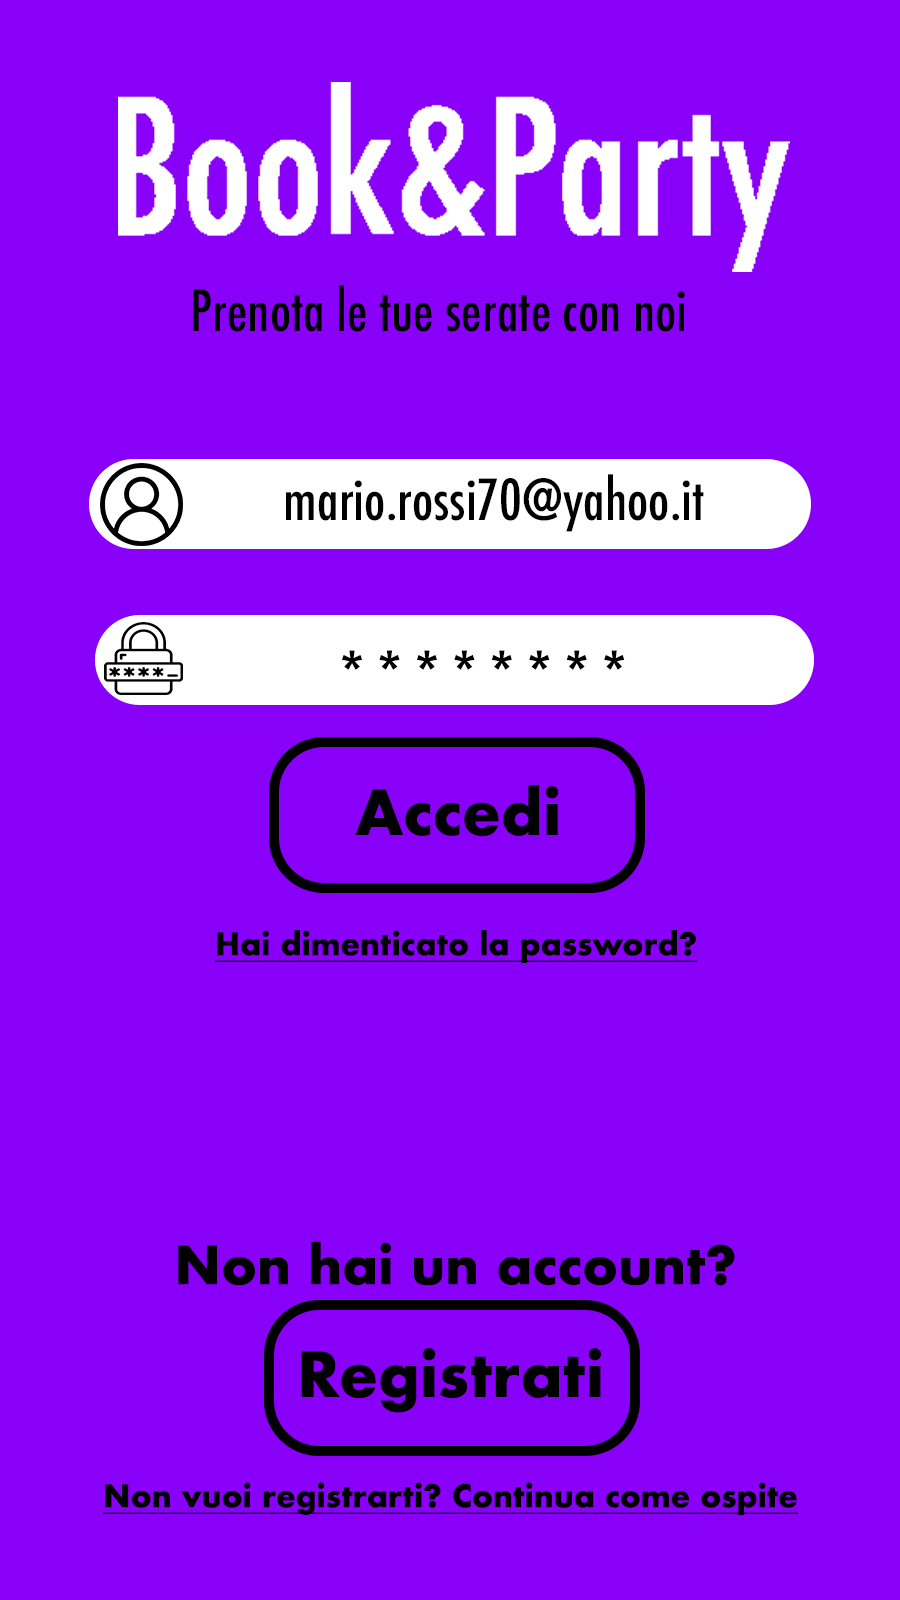
\includegraphics[width=5cm, height=10cm]{mockup/01-login.jpg}
    \label{fig:login}
\end{figure}

All'apertura dell'applicazione, all'utente gli verrà presentato la schermata soprastante, con 
il logo dell'app nella parte superiore e lo slogan dell'app subito sotto. Su questa pagina
l'utente potrà sia accedere tramite l'inserimento, negli appositi riquadri dotati di icon, 
la propria e-mail e password. 
 
Se l'utente non fosse registrato, gli sarà possibile farlo
cliccando il pulsante \textbf{Registrati}, il quale reindirizza alla pagina \ref{fig:registra}. 
 
In caso la password sia stata smarrita, si potrà cliccare sulla scritta sottostante il 
pulsante \textbf{accedi} (vedi \ref{sec:recPsw})

%registrazione
\section{Registrazione}
\begin{figure}[h]
    \centering
    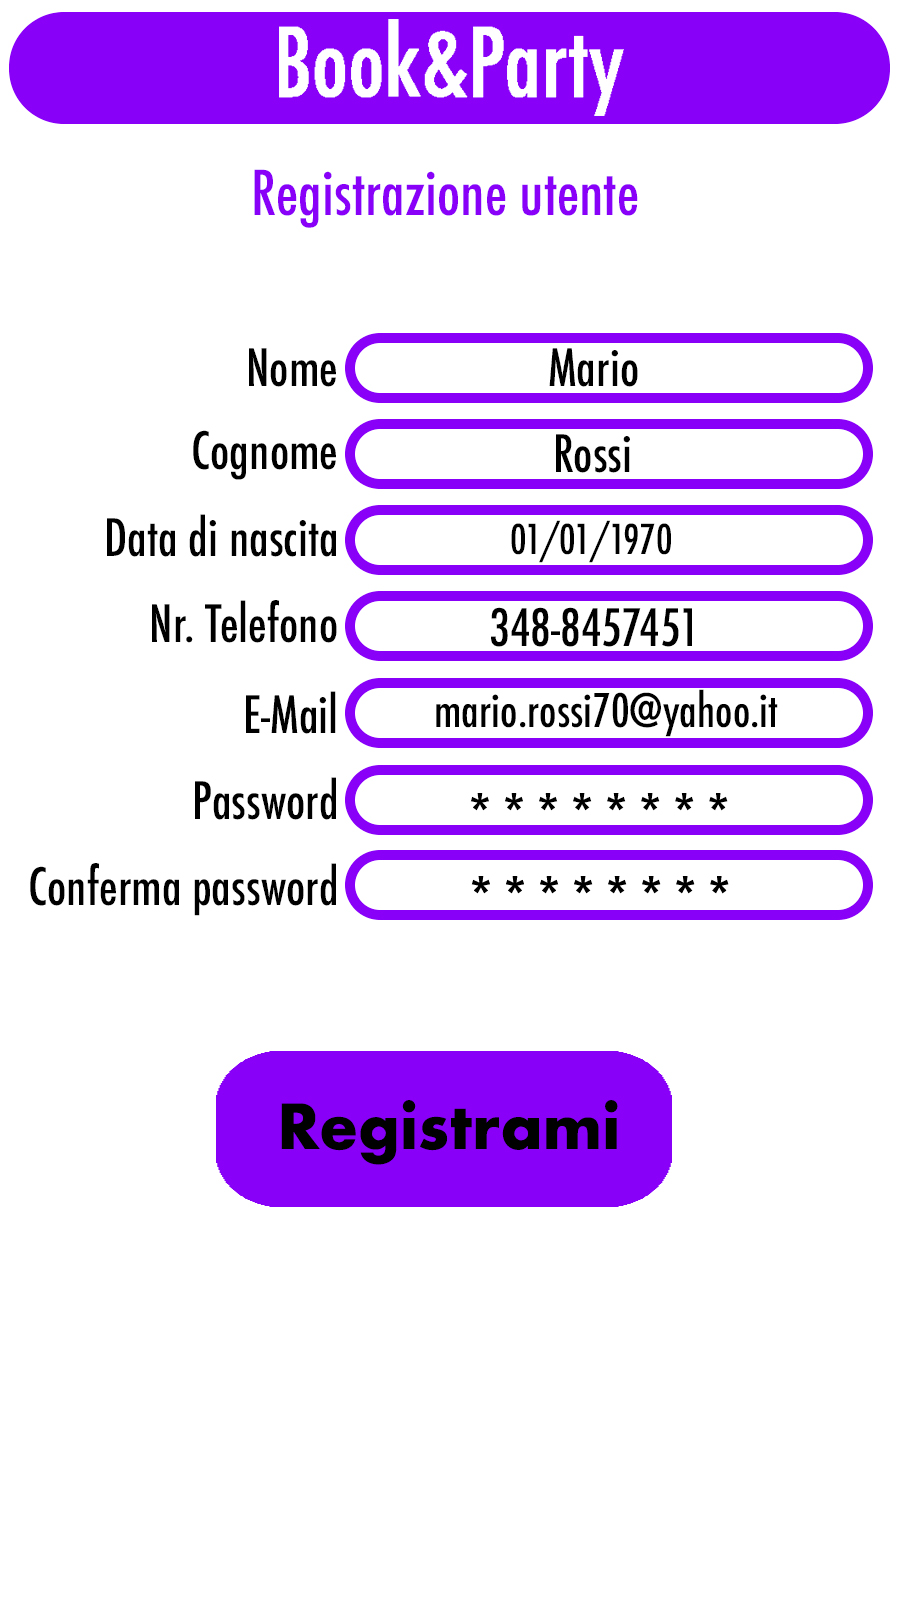
\includegraphics[width=5cm, height=10cm]{mockup/02-registrazione.jpg}
    \label{fig:registra}
\end{figure}

Al momento della registrazione l'utente deve inserire i propri dati (vedi 
\ref{sec:registrazione}) per la creazione dell'account

\newpage
%ricerca
\section{Ricerca}
\begin{figure}[h]
    \centering
    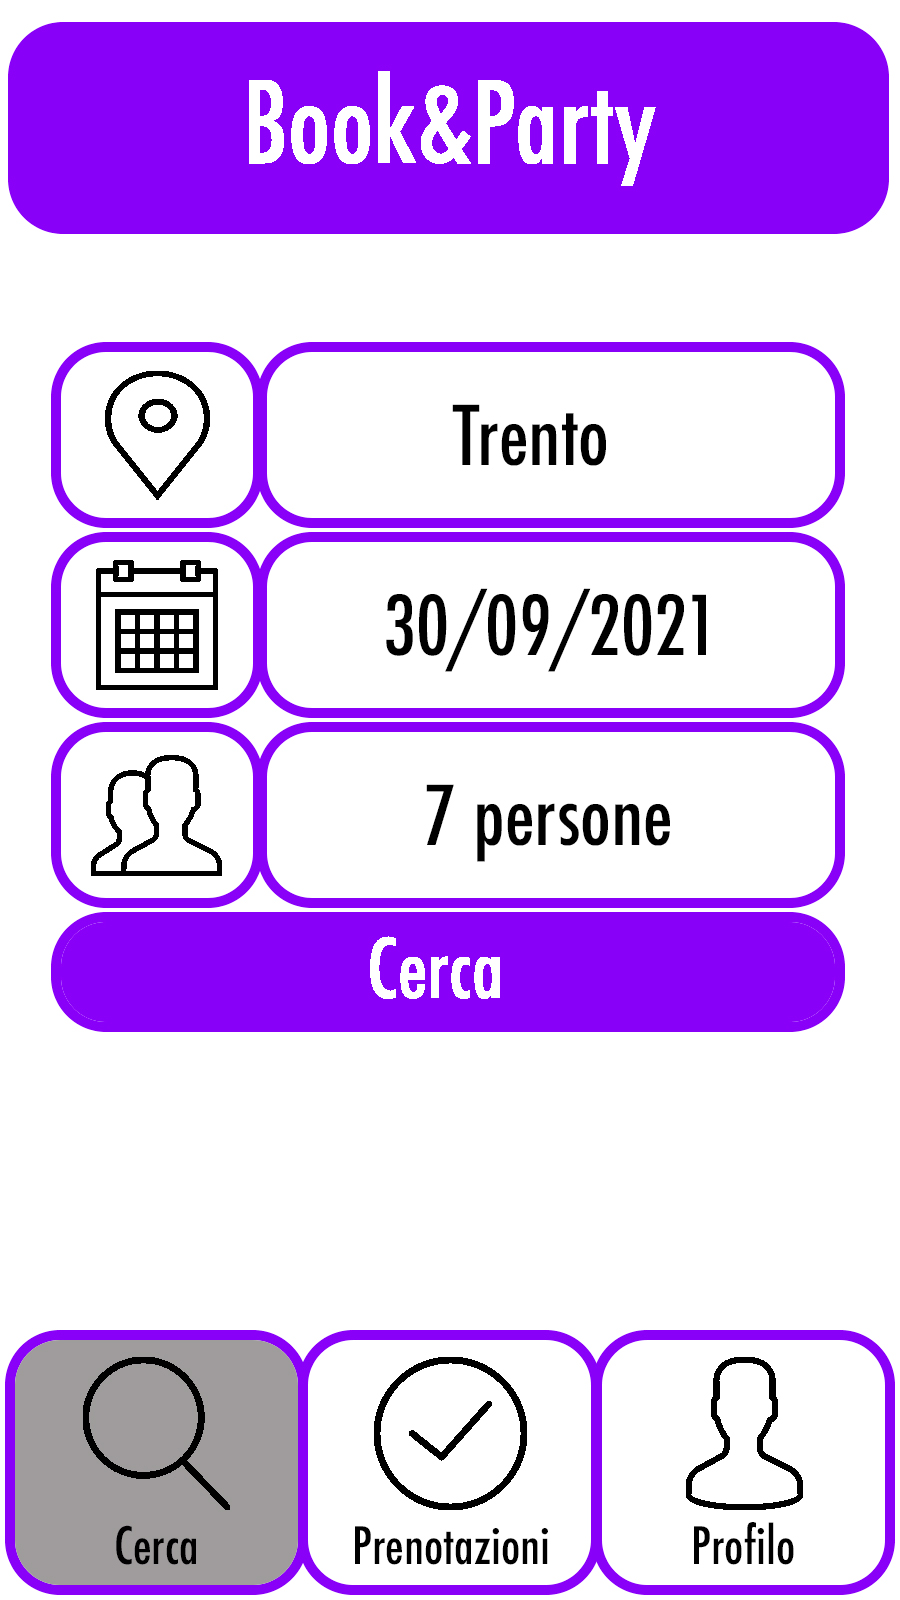
\includegraphics[width=5cm, height=10cm]{mockup/03-cerca-cliente.jpg}
    \qquad\qquad
    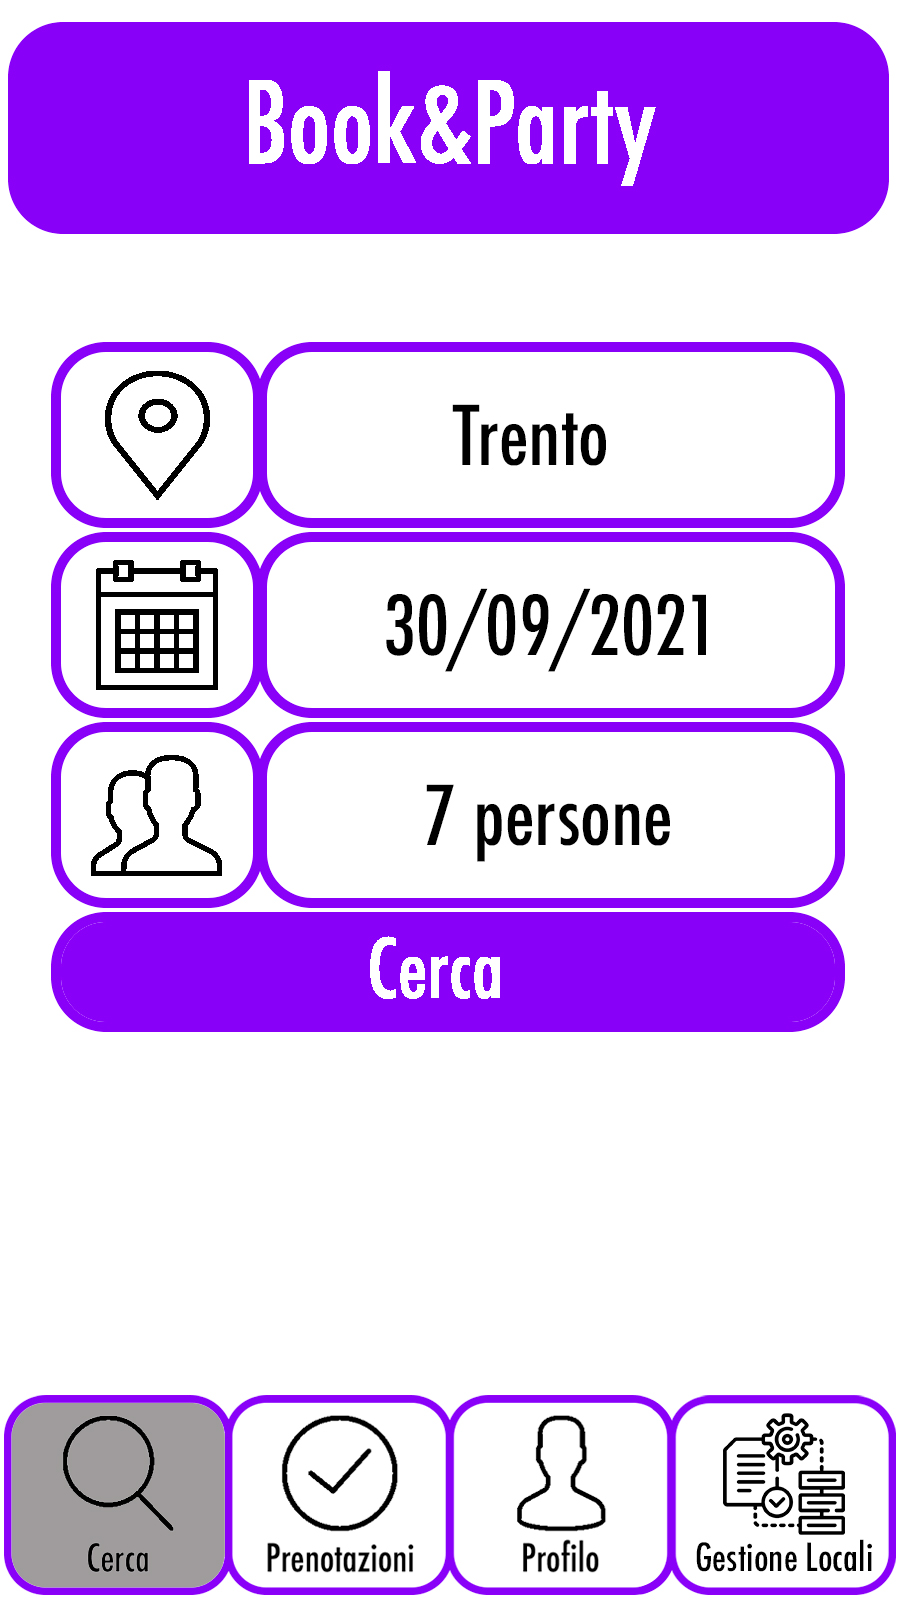
\includegraphics[width=5cm, height=10cm]{mockup/04-cerca-gestore.jpg}
    \label{fig:cerca}
\end{figure}

Dopo il login, l'utente viene indirizzato alla pagina di ricerca.
In questa pagina si possono visualizzare 3 sezioni per il \textbf{cliente} (cerca,
prenotazioni e profilo), 4 per il \textbf{gestore} (come cliente più gestione locali) e
solo la sezione \textbf{Cerca} per l'utente \textbf{non registrato}.
Nella sezione \textbf{Cerca} è possibile effettuare una ricerca inserendo il luogo 
desiderato e il numero di persone per le quali si sta prenotando. Cliccando sull'icona
\textbf{calendario} si aprirà un calendario pop-up sul quale l'utente potrà selezionare
una data. 
Cliccando sul pulsante \textbf{Cerca} verrà reindirizzato alla schermata dei risultati.

\newpage
%risultati ricerca
\section{Risultati ricerca}
\begin{figure}[h]
    \centering
    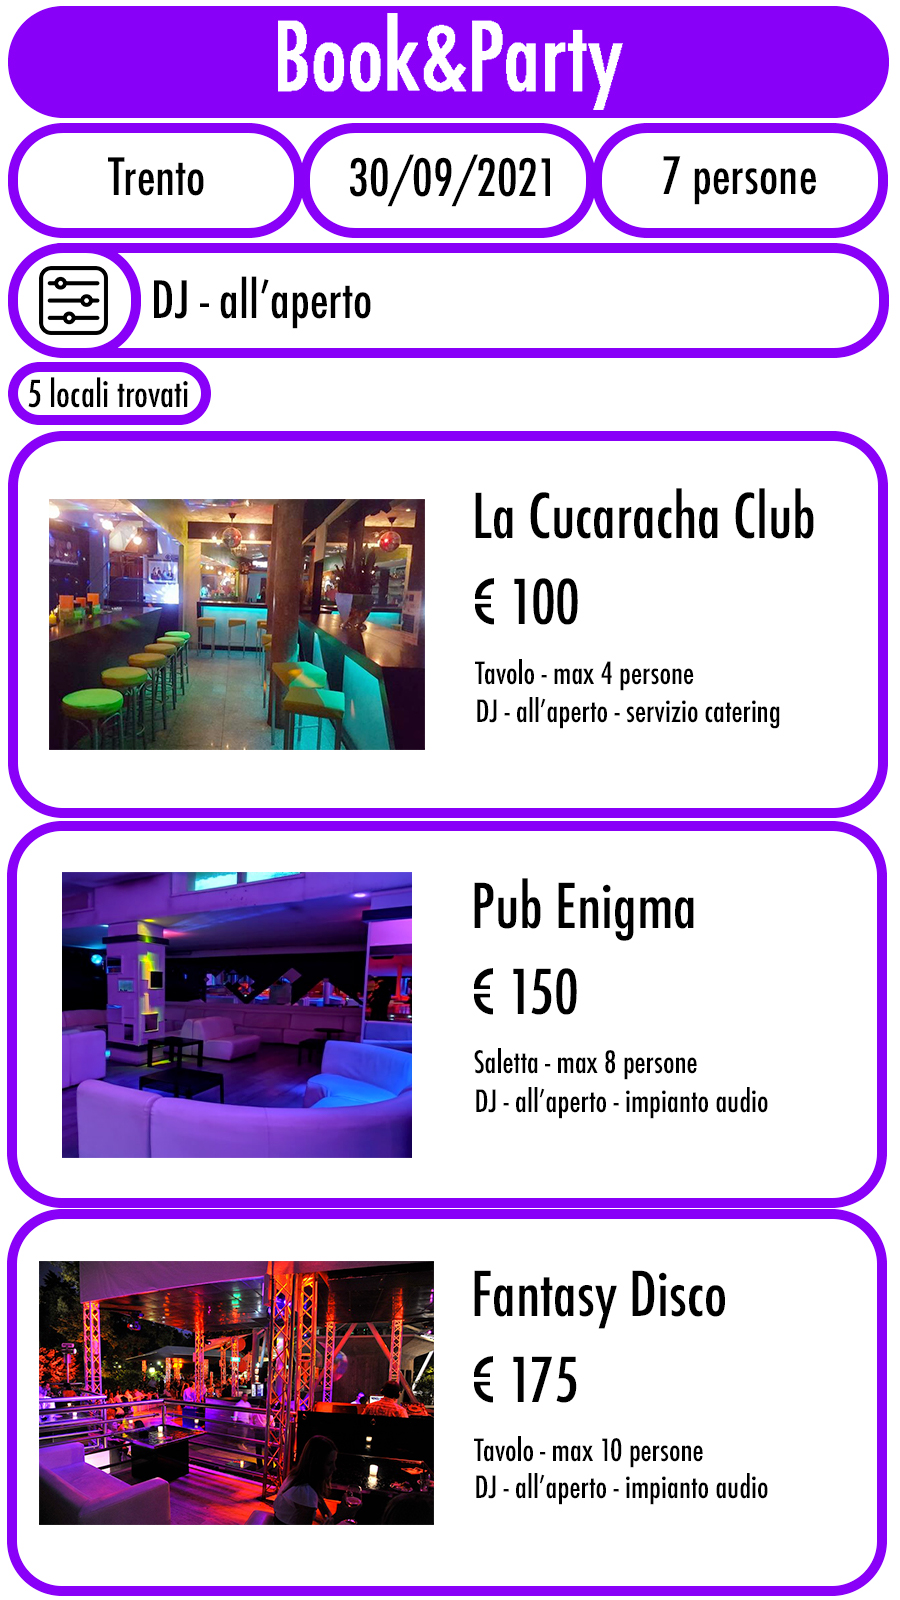
\includegraphics[width=5cm, height=10cm]{mockup/05-ricerche-filtri.jpg}
    \qquad\qquad
    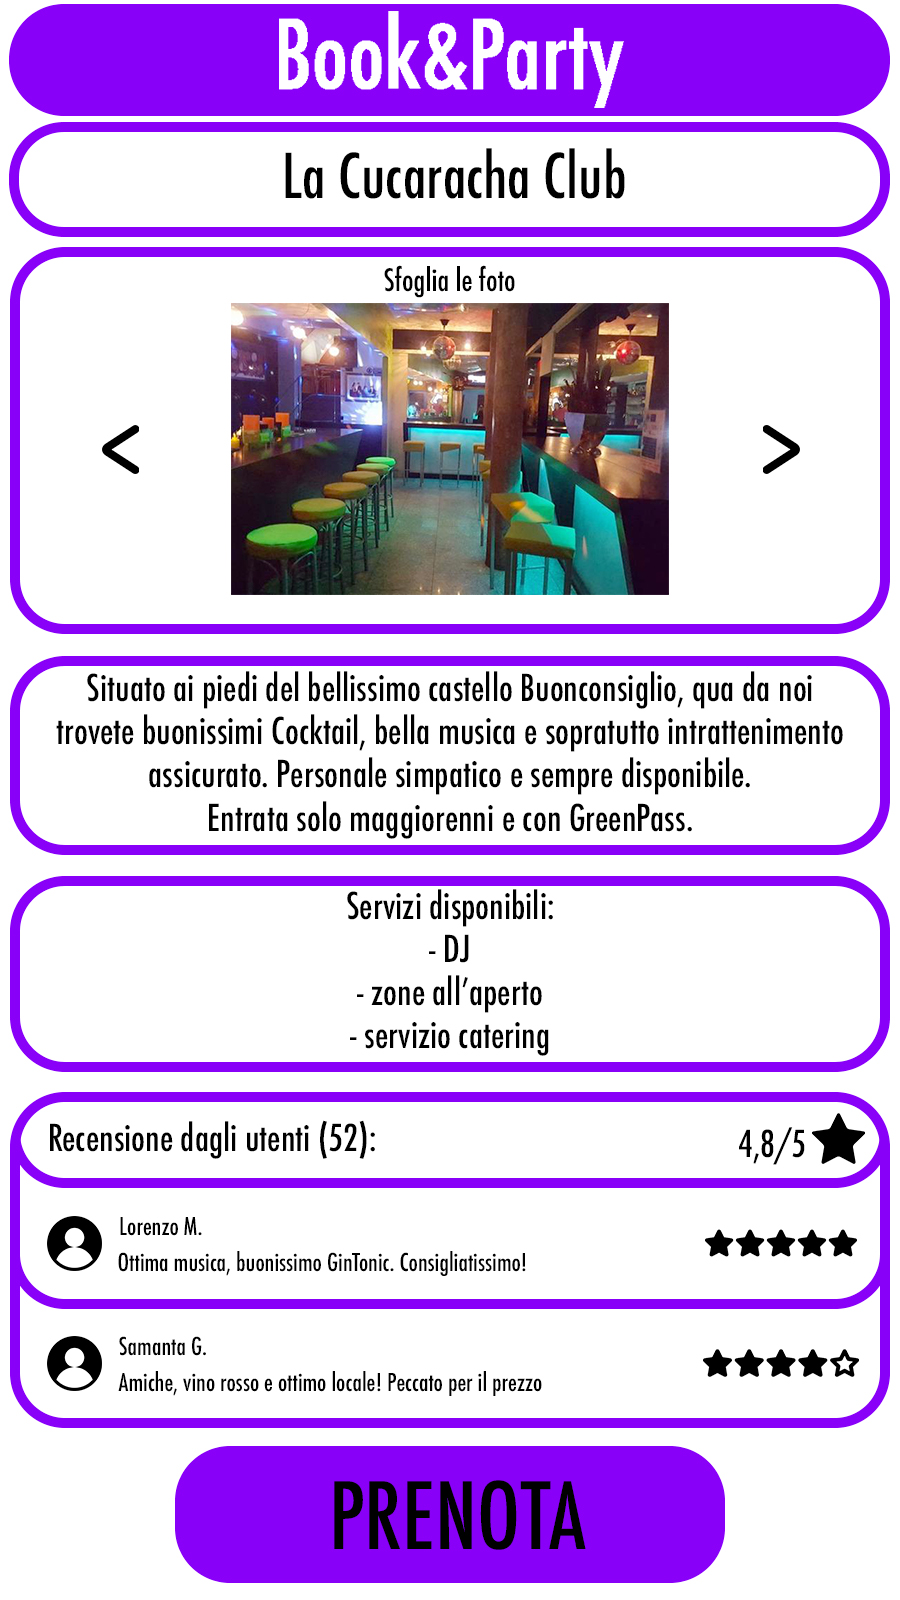
\includegraphics[width=5cm, height=10cm]{mockup/06-ricerca.jpg}
    \label{fig:risultati}
\end{figure}

Nella schermata dei risultati l'utente potrà usare il tasto \textbf{filtri} per fare una 
ricerca più specifica (vedi \ref{itm:filtri}). La pagina mostra il numero di risultati
ordinati in base al prezzo con una foto del locale, numero di posti massimi e servizi 
disponibili.
Cliccando su un locale l'utente passerà alla pagina con le informazione del locale 
selezionato.
Tale pagina conterrà foto, descrizione, servizi e commenti degli utenti. Il pulsante 
prenota porterà a una pagina di riepilogo contenente un elenco (vedi 
\ref{itm:recapPrenotazione}) ed un altro pulsante che indirizza alla pagina web di pagamento 
PayPal.

\newpage
%prenotazioni
\section{Prenotazioni}
\begin{figure}[h]
    \centering
    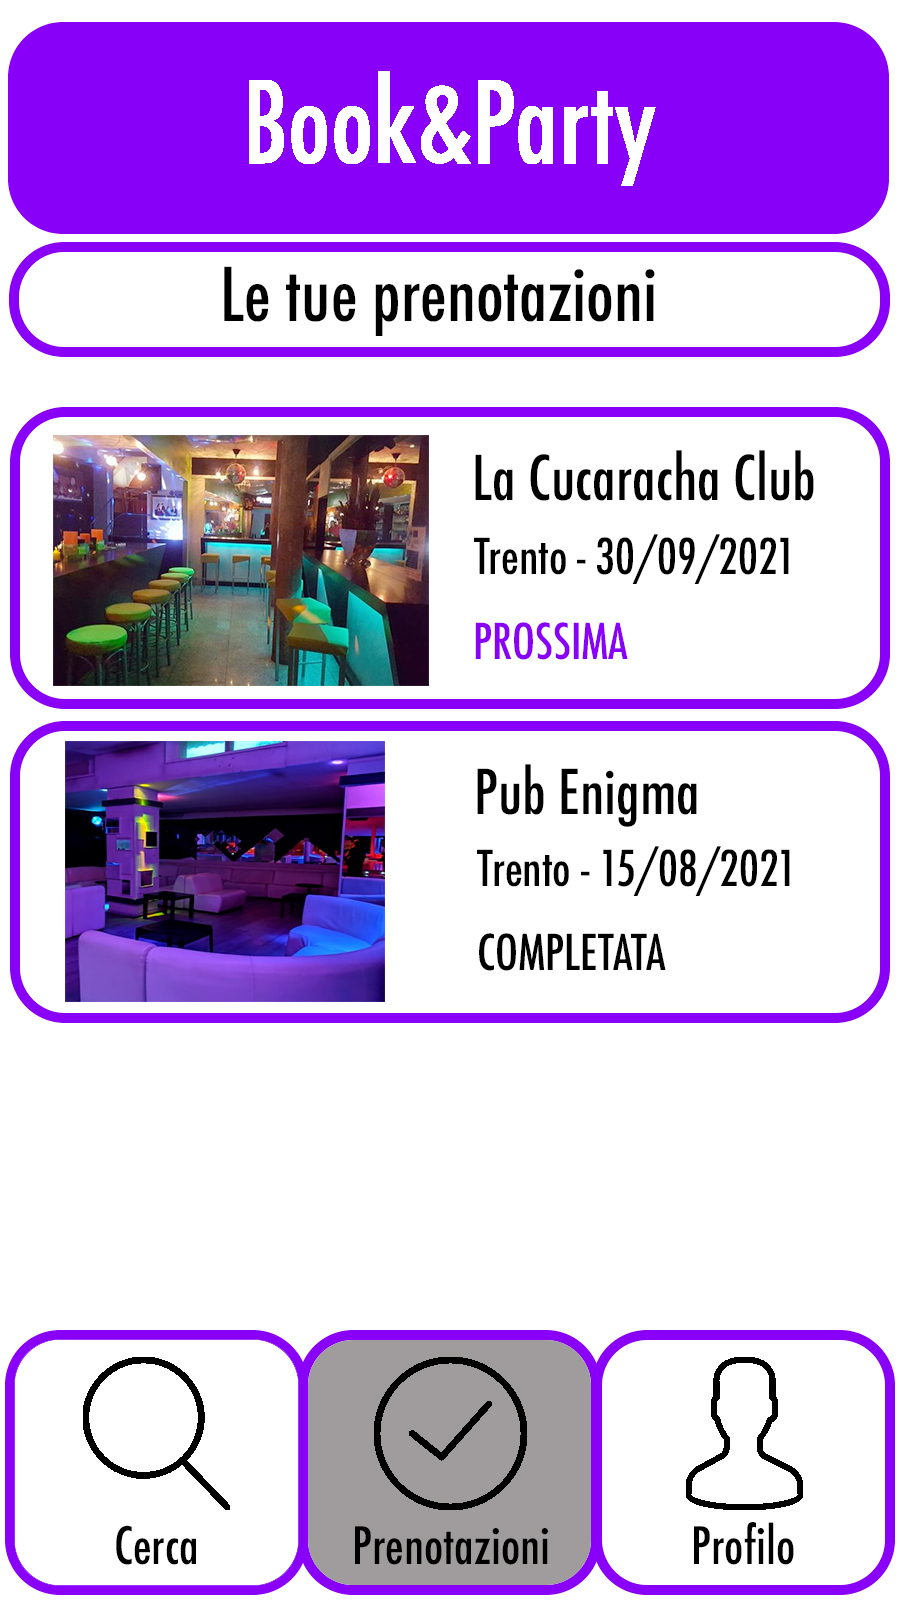
\includegraphics[width=5cm, height=10cm]{mockup/07-prenotazioni.jpg}
    \qquad\qquad
    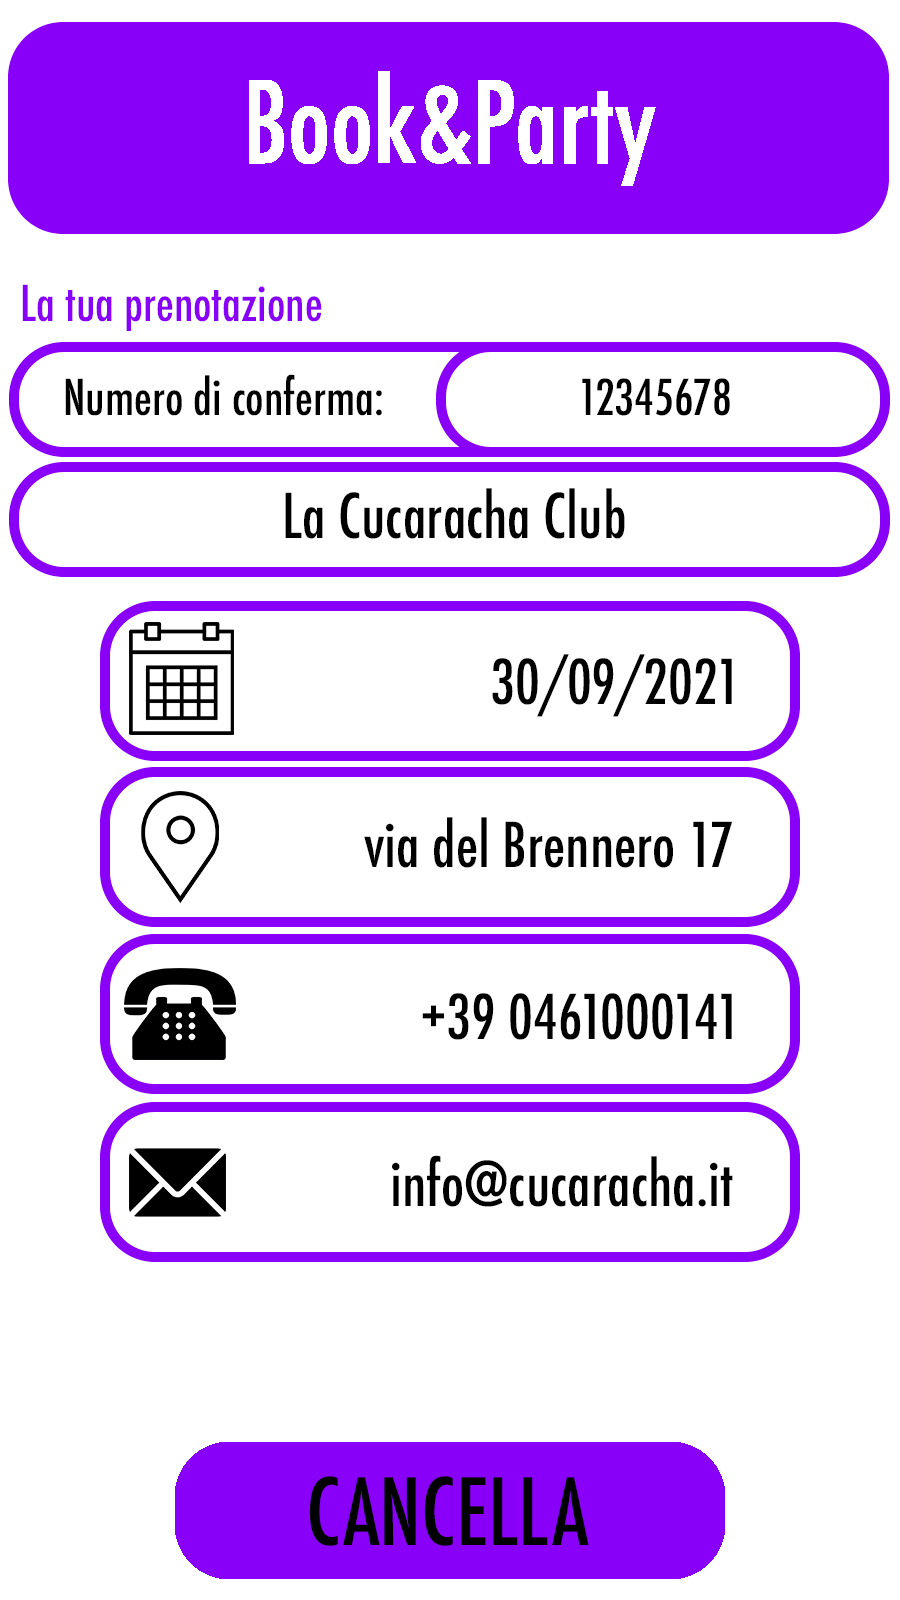
\includegraphics[width=5cm, height=10cm]{mockup/08-riepilogo-prenotazione.jpg}
    \label{fig:prenota}
\end{figure}

Andando nella sezione \textbf{Prenotazioni} il \textbf{cliente} viene indirizzato sulla pagina
\textbf{Le tue prenotazioni} dove potrà visualizzare tutte le prenotazioni effettuate. Potrà 
cliccare su una prenotazione per vedere le informazioni specifiche (vedi \ref{itm:prenotazione}). 
Cliccando su una prenotazione \textbf{completata} potrà lasciare una recensione al locale e invece 
per una prenotazione \textbf{prossima} avrà la possibilità di cancellarla.

\newpage
%profilo cliente
\section{Profilo Cliente}
\begin{figure}[h]
    \centering
    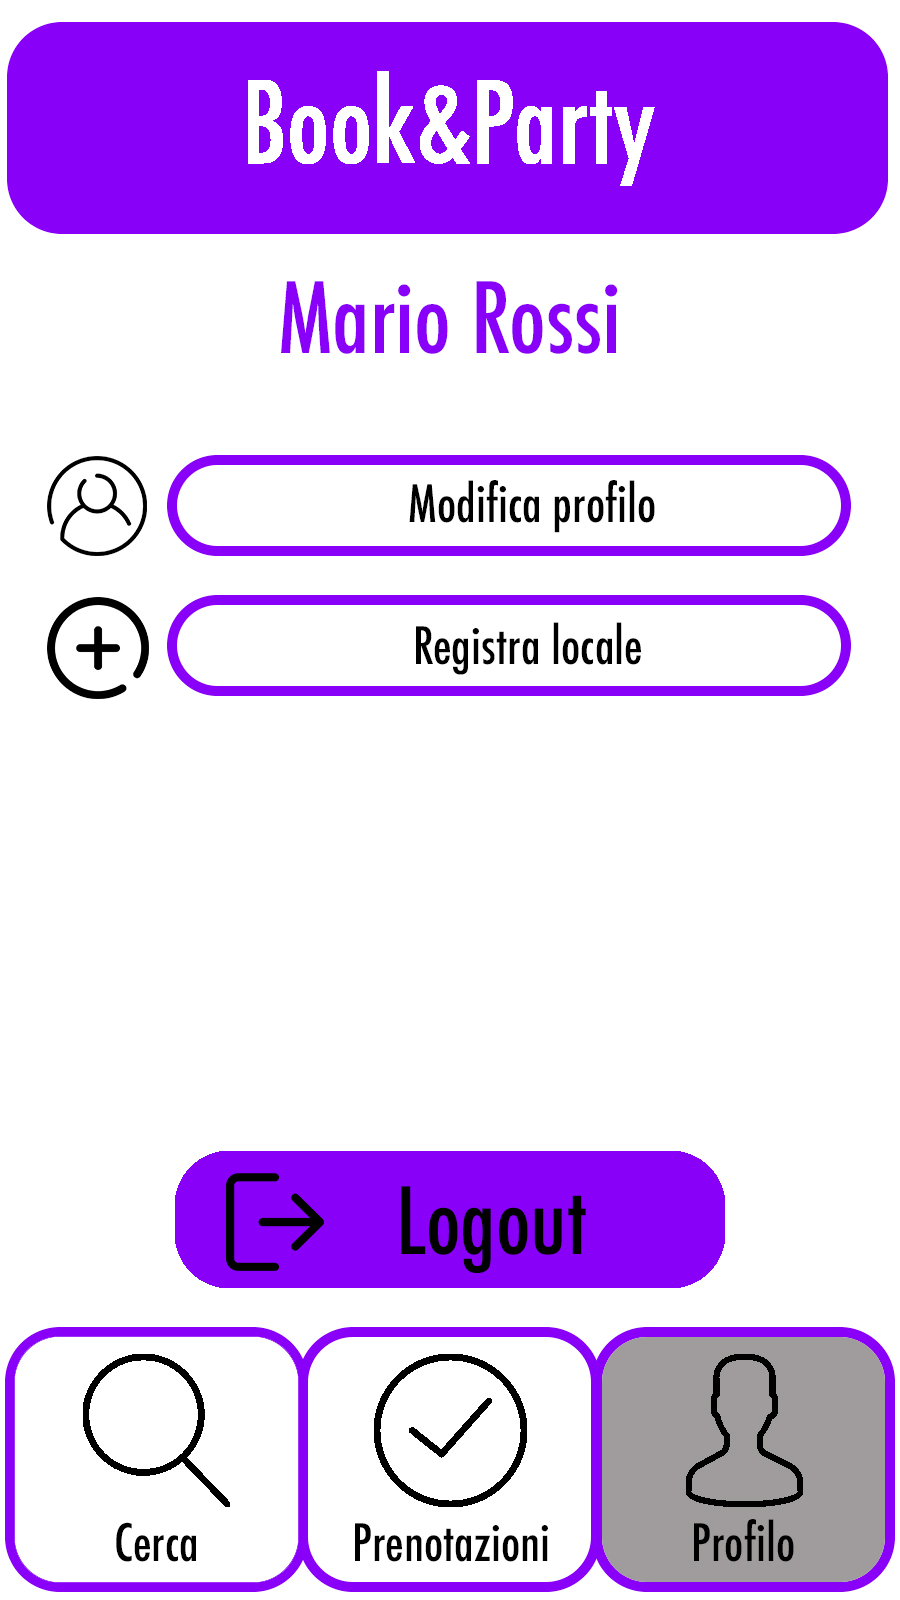
\includegraphics[width=5cm, height=10cm]{mockup/09-profilo-cliente.jpg}
    \label{fig:profiloCliente}
\end{figure}

Andando nella sezione \textbf{Profilo} il \textbf{cliente} (o il \textbf{gestore}) potrà 
modificare il proprio profilo cliccando su \textbf{Modifica profilo} (vedi 
\ref{sec:gesAccountCliente}). Cliccando il pulsante \textbf{Registra locale} il cliente 
verrà indirizzato alla pagina di registrazione del locale (simile a quella per registrarsi. Vedi 
\ref{itm:infoLocale}). Una volta aggiunto il primo locale, o eliminati tutti quelli in suo 
possesso, la barra delle sezioni cambierà per rispettare questo cambiamento di utente. In fine 
potrà cliccare sul pulsante \textbf{Logout} che lo riporterà alla pagina di login.

\newpage
%profilo locale
\section{Profilo \textcolor{red}{Locale}} \label{sec:proLocale}
\begin{figure}[h]
    \centering
    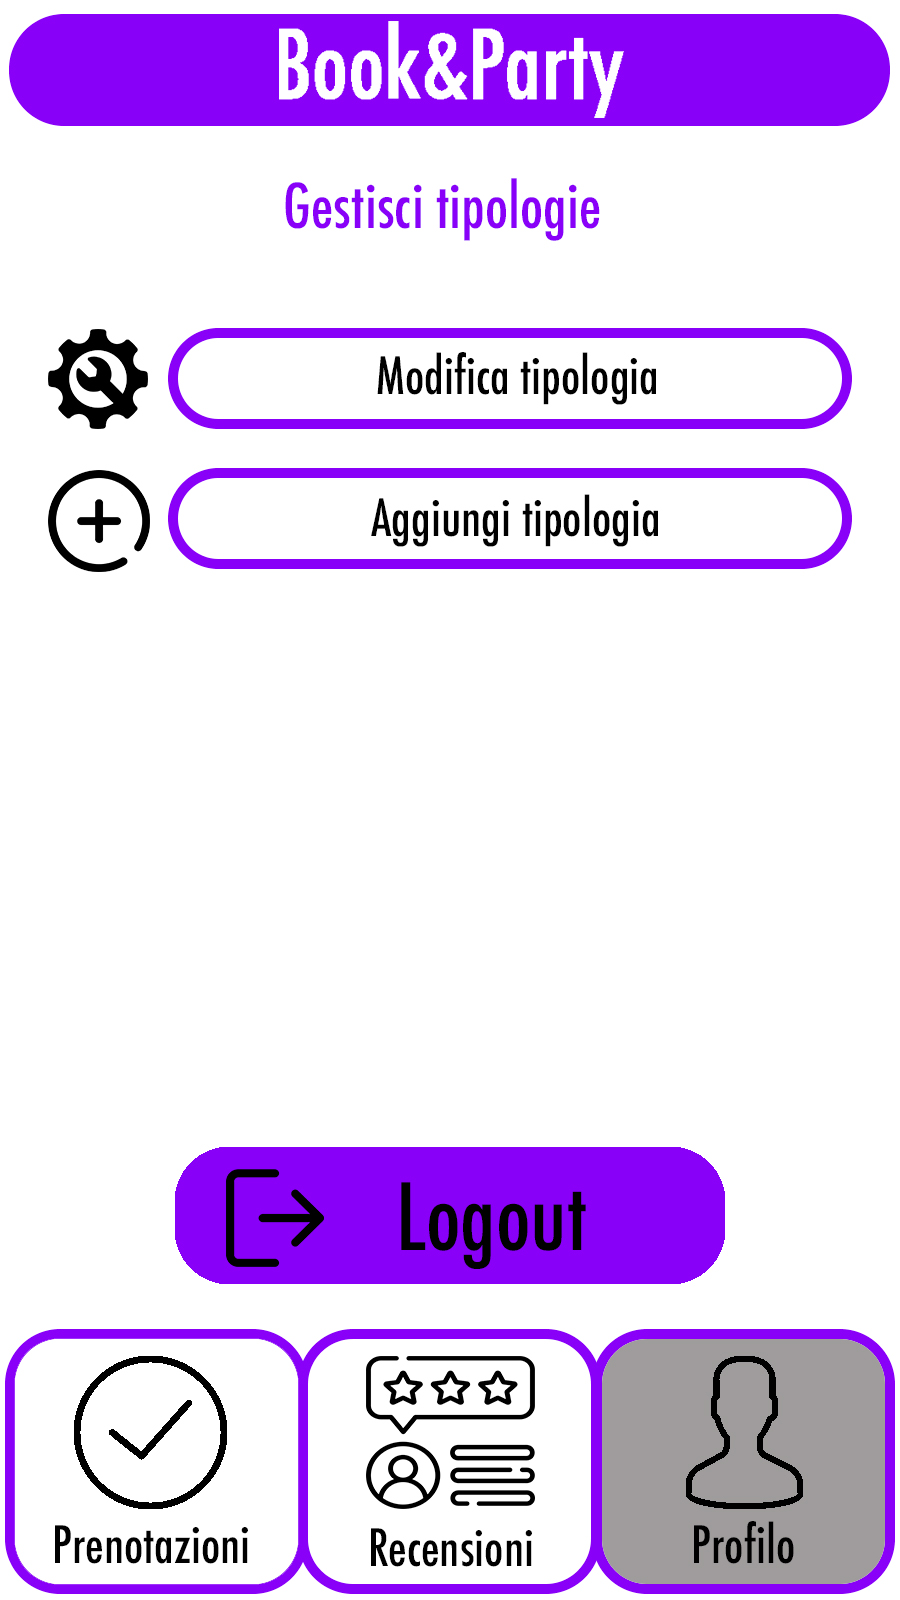
\includegraphics[width=5cm, height=10cm]{mockup/10-profilo-locale.jpg}
    \label{fig:profiloLocale}
\end{figure}

In questa schermata il locale ha la possibilità di modificare le tipologie già inserite, 
eliminarle (non possibile se n'è presente solo una), o aggiungerne.
Cliccando sul pulsante \textbf{Logout} verrà indirizzato alla pagina di login.

\newpage
%darkmode
\section{Dark mode}
\begin{figure}[h]
    \centering
    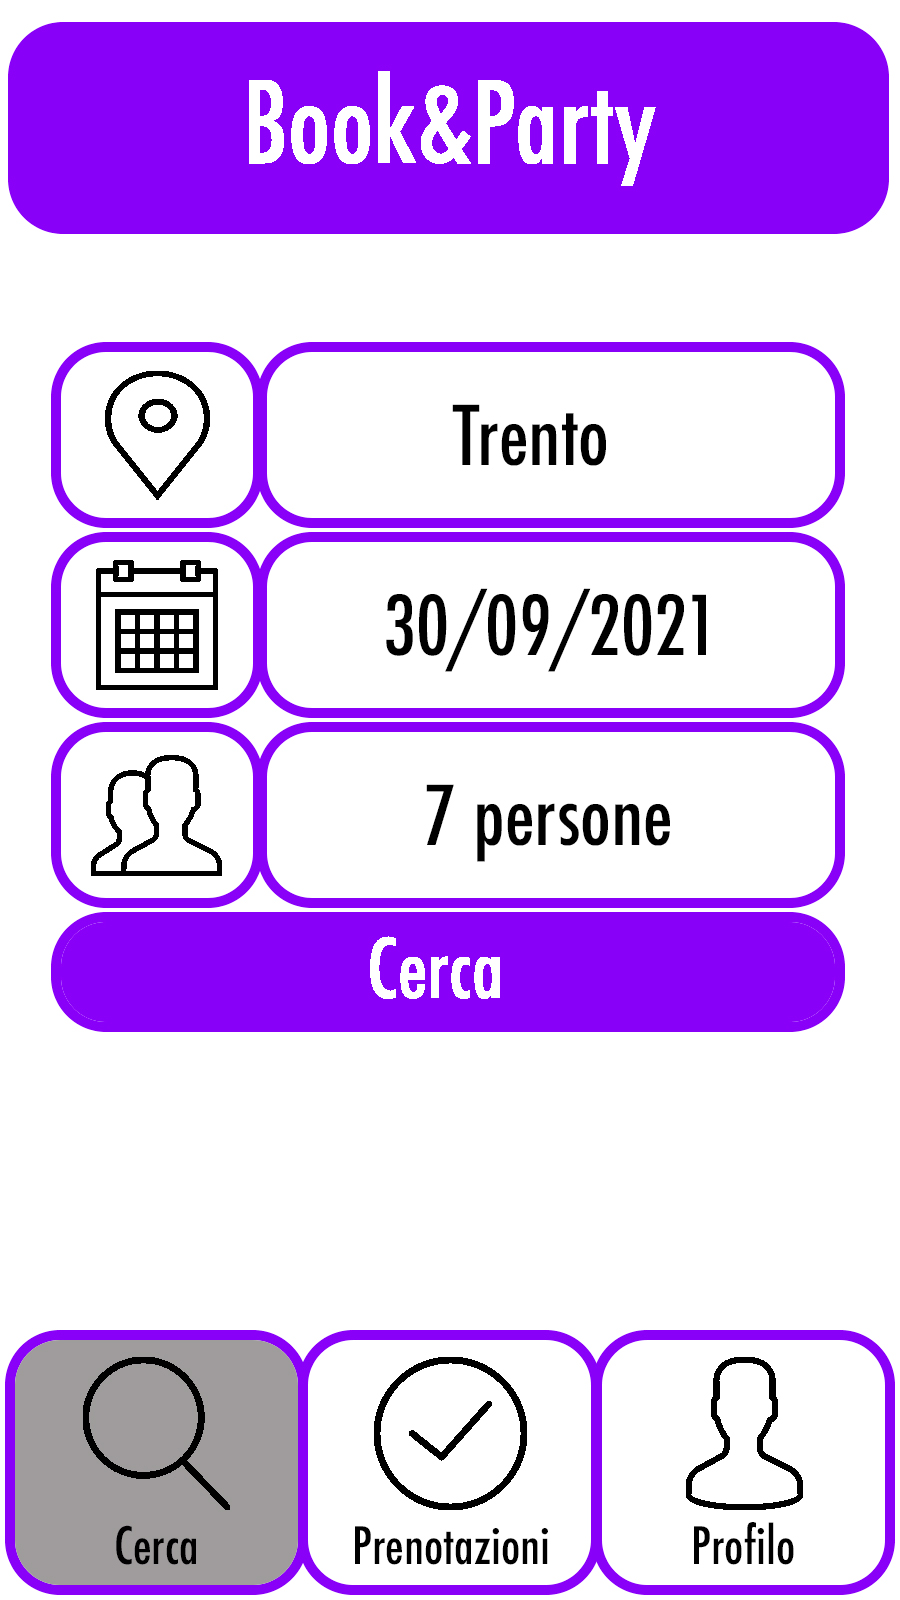
\includegraphics[width=5cm, height=10cm]{mockup/03-cerca-cliente.jpg}
    \qquad\qquad
    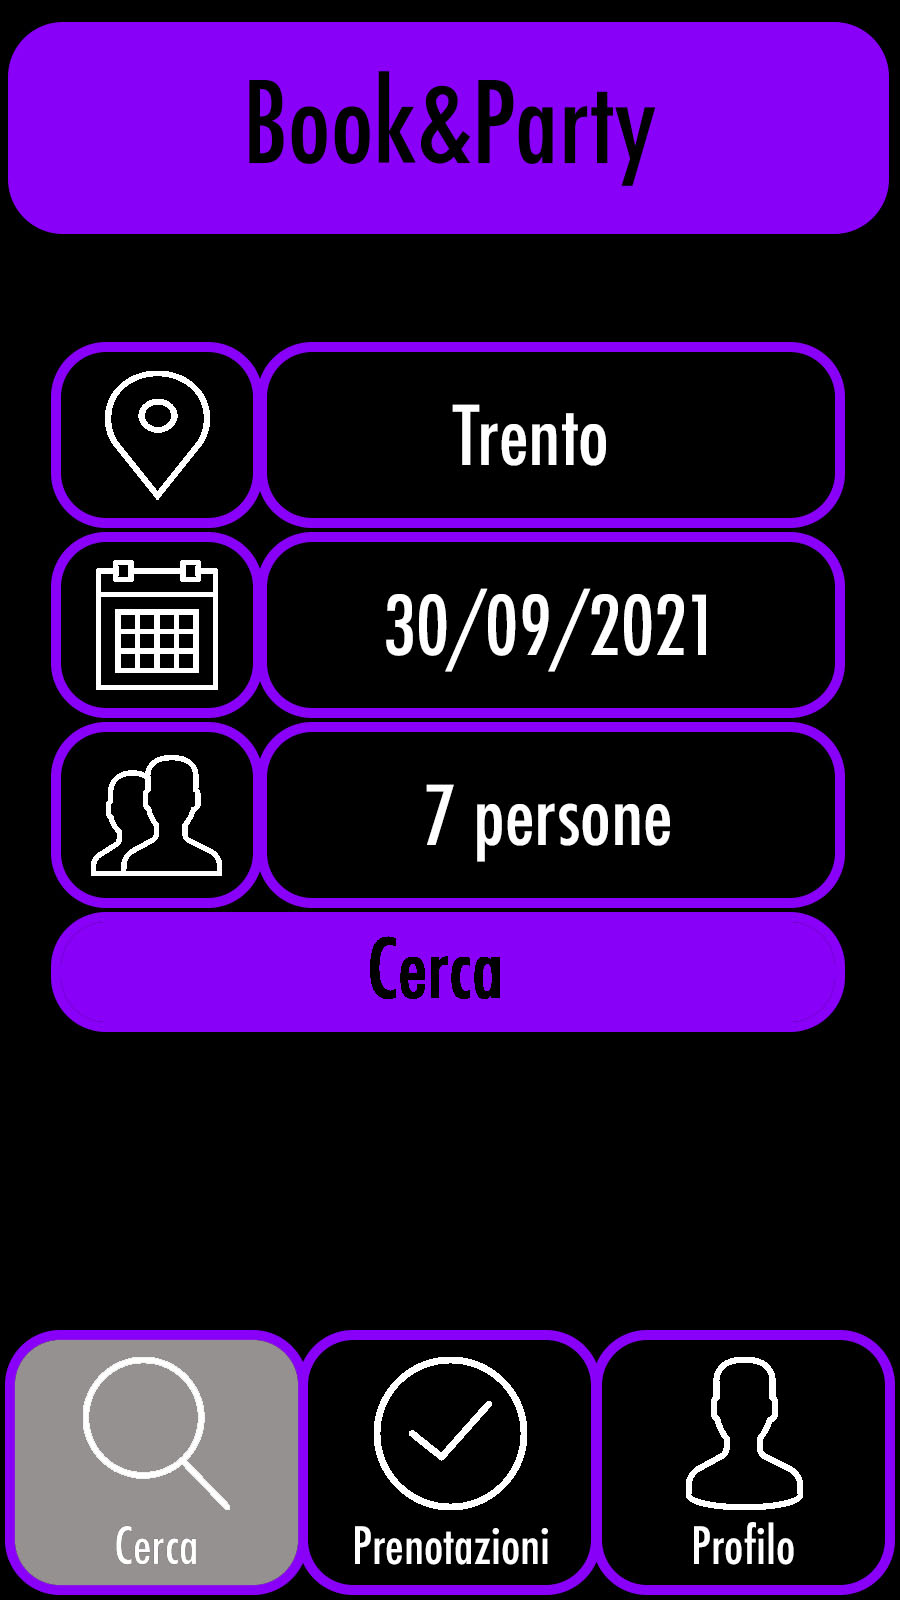
\includegraphics[width=5cm, height=10cm]{mockup/11-dark-mode.jpg}
    \label{fig:mode}
\end{figure}

Questa schermata serve a dare un esempio su come dovrà aprire l'applicazione se l'utente sarà
nella modalità \textbf{light mode} o in \textbf{dark mode}